\documentclass{article}

\usepackage[utf8]{inputenc}
\usepackage{url}
\def\UrlFont{\em}
\usepackage{indentfirst}

\title{Trabalho de Visão Relatório}
\author{Felipe Leivas Machado - 262528 \and Priscila Cavalli Rachevsky - 261573 }

\usepackage{natbib}
\usepackage{graphicx}
\usepackage{capt-of}

\begin{document}

\maketitle

\section{Introdução}
    A partir de uma imagem com linhas que representavam os eixos x e y de um plano cartesiano e uma parábola precisava a plotar essas linhas novamente, garantindo que os eixos eram perpendiculares e garantindo que a parábola seguisse uma equação de segundo grau. Para isso, precisou seguir esses passos:
   \begin{itemize}
       \item Extrair uma imagem de bordas
       \item Identificar os eixos X e Y
       \item Remover os eixos
       \item Identificar a parábola
   \end{itemize}
\section{Implementação}
   \subsection{Extrair uma imagem de bordas}
   Primeiramente, a imagem foi transformada para ter apenas tons cinza. Então, se aplicou o filtro Gaussiano com kernel tamanho 7 para diminuir eventuais ruídos. Dessa forma, aplicou-se linearização, no qual o linear tinha o valor de 143.
   \begin{figure}[h!]
   \centering
    \subfigure
        {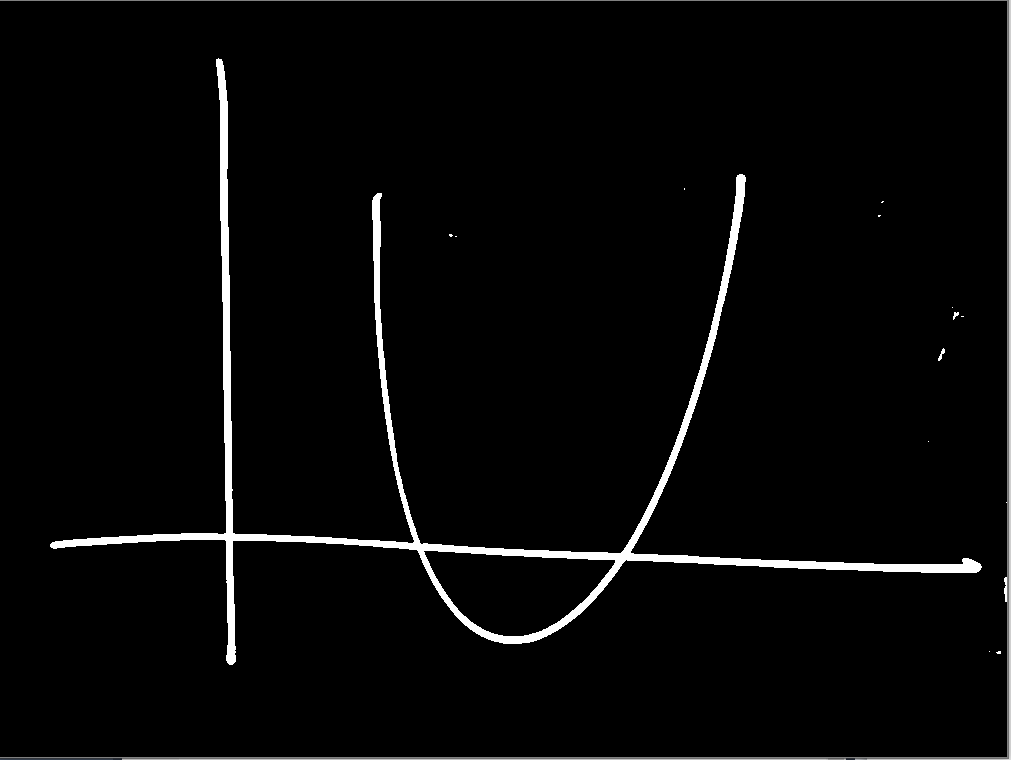
\includegraphics[scale=0.17]{exemplo1_edge.PNG}}
    \subfigure
        {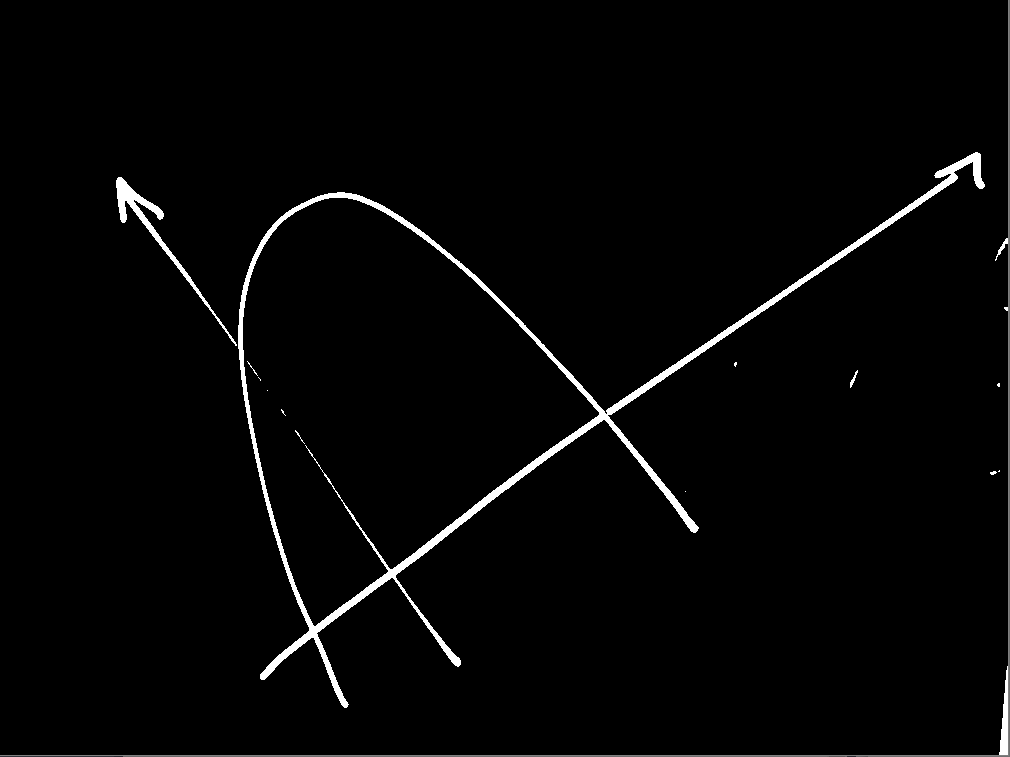
\includegraphics[scale=0.17]{exemplo2_edge.PNG}}
    \subfigure
        {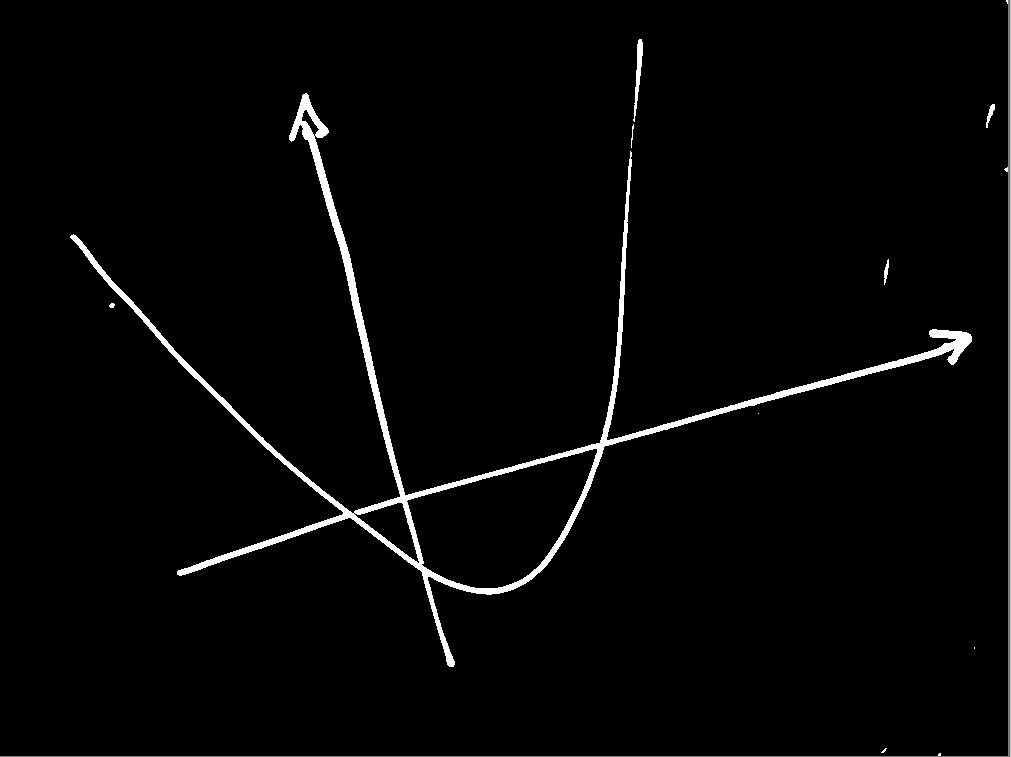
\includegraphics[scale=0.17]{exemplo3_edge.PNG}}
    \caption{Imagens de bordas}
    \end{figure}

   \subsection{Identificar os eixos X e Y}
   Usou-se Hough para identificar as linhas maiores, tamanho mínimo de 300 pixels e no máximo 50 de gap. Então, identificou-se que as linhas eram eixo X quando a diferença entre seus 2 pontos era maior no x do que no y, ou seja, (x1 - x2)² > (y1 - y2)², caso contrário, a linha representava o eixo y.
   \subsection{Remover os eixos}
   \subsection{Identificar a parábola}

\end{document}
